\documentclass[11pt,a4paper]{article}

% Define page geometry
\usepackage{geometry}
\geometry{left=2.2cm,
	right=2.2cm,
	top=2.2cm,
	bottom=2cm} % Page margins
\parskip 0.15cm % Paragraph spacing
\setlength{\parindent}{0cm} % No paragraph indenting

\usepackage{pdflscape} % Landscape pages

% Text formatting
\usepackage[T1]{fontenc} % Set font

\usepackage{lineno} % Line numbers

\usepackage{amssymb} % Symbols

\linespread{1.5} % Linespacing

\usepackage{xcolor}
\newcommand{\todo}[1]{\textcolor{red}{\textbf{#1}}}  % todonote

% Tables
\usepackage{multirow}
\setlength{\tabcolsep}{4pt} % Default table column sep width 

% Image handling
\usepackage{graphicx} 

\graphicspath{ {img/} } % Define image path

\usepackage{float} % Precise figure location

% Bibliography management
\usepackage[style=authoryear, natbib=true, backend=biber]{biblatex}
\addbibresource{phenology.bib}

% Links within document, nice figure formatting
\usepackage[breaklinks]{hyperref}
\definecolor{links}{RGB}{0,0,0}
\hypersetup{
	breaklinks,
	colorlinks=true,
	linkcolor=links,
	anchorcolor=links,
	citecolor=links,
	filecolor=links,
	menucolor=links,
	runcolor=links,
	urlcolor=links,
	pdfauthor={John L. Godlee}
}
\def\subsectionautorefname{section}
\def\subsubsectionautorefname{section}

\newcommand{\beginsupplement}{%
	\setcounter{table}{0}
	\renewcommand{\thetable}{S\arabic{table}}%
	\setcounter{figure}{0}
	\renewcommand{\thefigure}{S\arabic{figure}}%
	}
   
% Variables
\input{out/vars.tex}

% Title
\newcommand{\titletext}{Phenology and diversity in Zambia}

\begin{document}

{\Large{Title: \titletext{}}}

Authors: Godlee J. L.\textsuperscript{1}, Ryan C. M.\textsuperscript{1}, Siampale A.\textsuperscript{2}, Dexter K. G.\textsuperscript{1,3}

\textsuperscript{1}School of GeoSciences, University of Edinburgh, Edinburgh, United Kingdom \\
\textsuperscript{2}Forestry Department Headquarters - Ministry of Lands and Natural Resources, Cairo Road, Lusaka, Zambia \\
\textsuperscript{3}Royal Botanic Garden Edinburgh, Edinburgh, EH3 5LR, United Kingdom \\

\vspace{1em}
Corresponding author:

John L. Godlee

johngodlee@gmail.com

School of GeoSciences, University of Edinburgh, Edinburgh, United Kingdom

\section*{Acknowledgements}

\section*{Author constribution statement}

JLG conceived the study, conducted the analysis, and wrote the first draft of the manuscript. AS coordinated plot data collection in Zambia, and initial data management. All authors contributed to manuscript revisions. 

\section*{Data accessibility statement}

The data used in this study are held by the Zambian Integrated Land Use Assessment Project (ILUA-II), and were cleaned by the SEOSAW project (Socio-ecological Observatory for Southern African Woodlands). The data are not publicly available at the time of submission due to privacy concerns surrounding plot location, but can be requested from the corresponding author. An anonymised version will be made available in a data repository following review.

\newpage{}
\linenumbers

{\Large{Blinded Main Text File}}\\
{\Large{Title: \titletext{}}}

\section*{Abstract}

\section{Introduction}

The seasonal timing and duration of tree leaf production (land-surface phenology) in dry deciduous savannas directly influences ecosystem processes. Leaf Area Index (LAI), the leaf area per unit ground area, and the green-ness of leaves are both tightly coupled with photosynthetic activity and therefore Gross Primary Productivity (GPP) \citep{Gu2003, Penuelas2009}. Directional shifts in GPP influence the accumulation rate of woody biomass, and affect the delicate balance between tree and grass co-occurrence in these ecosystems \citep{Stevens2016}, with potential consequences for transition between closed-canopy forest and open savanna. From a conservation perspective, within deciduous savannas, those with a longer growth period support a greater diversity and abundance of wildlife, particularly bird species but also browsing mammals \citep{Cole2015, Araujo2017, Morellato2016, Ogutu2013}. Extreme weather patterns as a result of climate change are leading to shorter but more intense leaf production cycles in these ecosystems which are already close to the edge of their climatic envelope, with severe negative consequences anticipated for biodiversity \citep{Bale2002}. Understanding the determinants of seasonal patterns of tree leaf production in dry deciduous savannas can provide valuable information on spatial variation in vulnerability to climate change, and help to model their contribution to land surface carbon cycle models under climate change.

Previous studies have shown that diurnal temperature variation and precipitation are the primary determinants of tree phenological activity in water-limited savannas. At regional spatial scales, savanna phenological activity can be predicted using only climatic factors and light environment \citep{Adole2018a}, but local variation exists in leaf production cycles which cannot be attributed solely to abiotic environment. It has been repeatedly suggested that information on biotic environment play a larger role in predicting land-surface phenology \citep{Adole2018b, Jeganathan2014, Fuller1999}, but implementation is most often limited to coarse ecoregions or functional vegetation types, which lack the fine-scale resolution which can take advantage of state-of-the-art earth observation data \citep{}.

Tree species vary in their life history strategy with regards to the timing of leaf production \citep{Fenner1998, Cole2017, Medina1994}. More conservative species (i.e. slower growing, robust leaves, denser wood) tend to initiate leaf production (green-up) before rainfall has commenced, and persist after the rainy season has finished, despite having lower cumulative GPP during the growing season, while more resource acquisitive species and juvenile individuals tend to green-up during the rainy season, and create a dense leaf-flush during the mid-season peak of growth \citep{}. It has been suggested that this variation in leaf phenological activity between species is one aspect by which increased tree species richness causes an increase in ecosystem-level productivity in deciduous savannas \citep{}. It has also been suggested that species richness could buffer ecosystem phenology against climate warming effects \citep{Parmesan2007}. Building on research linking biodiversity and ecosystem function, one might expect that an ecosystem with a greater diversity of tree species might be better able to maintain consistent leaf coverage for a longer period over the year, as species vary in their optimal growing conditions due to niche complementarity, whereby coexisting species vary in their occupation of niche space due to competitive exclusion \citep{}.

In the water-limited savannas such as those found in large areas of southern Africa \citep{}, the ability of conservative tree species to maintain consistent leaf coverage in the upper canopy strata over the growing season, but particularly at the start and end of the growing season, may provide facilitative effects to other tree species and juveniles occupying lower canopy strata that are less well-adapted to moisture-limiting conditions, but are more productive, by providing shade and influencing below ground water availability through hydraulic lift \citep{}. 

Variation in tree species composition, as well as species richness, is also expected to have an effect on savanna phenology in southern Africa. Savannas of a number of different types (species composition and structure) are found across southern Africa, but these are often poorly differentiated in regional-scale phenological studies \citep{} resulting in a dearth of information on the phenological behaviour of different woodland types. As our ability to remotely sense tree species composition improves, it allows us to create more tailored models of the carbon cycle which incorporate not only climatic factors, but also biotic factors which govern productivity. We therefore need to understand how species composition and biodiversity metrics affect land-surface phenology. 

While rates of greening and senescence at the start and end of the growing season measure the synchronicity of the synchronicity of plant growth, the lag between the onset of the plant growth and the onset of precipitation measure the reactivity of plant activity to precipitation. Both synchronicity and reactivity are expected to vary according to tree species composition. High synchronicity (high rate of greening and senescence) is expected to occur in tree communities with low diversity, as individuals from the same species are more likely to green-up together and exhibit reduced niche complementarity regarding green-up. Greater lag is expected to occur in tree communities with greater diversity, as the likelihood of including a species which greens earlier increases as the species pool grows.

In the deciduous woodlands of Zambia, a highly pronounced single wet-dry season annual oscillation is observed across the majority of land area, with local exceptions in some mountainous areas \citep{}. Variation in leaf phenological activity across the country has a large influence on annual GPP. Using Zambia as a case study, we can expect similar response from deciduous woodlands across southern Africa, with important consequences for the global carbon cycle \citep{}. 

While cumulative leaf production across the growing season may be the most important aspect of leaf phenology for GPP, other phenological metrics may be more important for ecosystem function and habitat provision for wildlife. Periods of green-up and senescence which bookend the growing season are key times for invertebrate reproduction \citep{}, soil biotic activity \citep{} and herbivore browsing activity \citep{}. Pre-rainy season green-up in water-limited savannas provides a valuable source of moisture and nutrients before the rainy season, and can moderate the understorey microclimate, increasing humidity, reducing UV exposure, and moderating diurnal oscillations in temperature, reducing ecophysiological stress which can lead to mortality during the dry season. An increase in the time between leading tree growth and the onset of seasonal rains provides a buffer to stressful dry season climatic conditions and wildlife activity. A slower rate of green-up caused by tree species greening at different times provides an extended period of bud-burst, thus maintaining the important food source of nutrient rich young leaves for longer \citep{}. 
 
In this study we contend that, across Zambian deciduous savannas, tree species diversity and composition influence three key measurable aspects of the tree phenological cycle: (1) the rates of greening and senescence at the start and end of the seasonal growth phase, (2) the overall length of the growth period, and (3) the lag time between green-up/senescence and the start/end of the rainy season. It is hypothesised that: (H\textsubscript{1}) due to variation among species in minimum viable water availability for growth, plots with greater tree species richness will exhibit slower rates of greening and senescence as different species green-up and senesce at different times. We expect that: (H\textsubscript{2}) in plots with greater species richness the start of the growing season will occur earlier in respect to the onset of rain due to an increased likelihood of containing a species which can green-up early, facilitating other species to initiate the growing season. We hypothesise that: (H\textsubscript{3}) plots with greater species richness will exhibit a longer growth period and greater cumulative green-ness over the course of the growth period, due to a higher resilience to variation in water availability, acting as a buffer to ecosystem-level productivity. Finally, we hypothesise that: (H\textsubscript{4}) irrespective of species diversity, variation in tree species composition and vegetation type will cause ecologically important variation in the phenological metrics outlined above. 

\section{Materials and methods}

\subsection{Data collection}

We used plot-level data on tree species diversity across \nSites{} sites from the Zambian Integrated Land Use Assessment Phase II (ILUA-II), conducted in \censusDate{} \citep{Mukosha2009, Pelletier2018}. Each site consisted of four 20x50 m (0.2 ha) plots positioned in a square around a central point, with a distance of 500 m between each plot (\autoref{schematic}). The original census contained \nTotalSites{} sites, which was filtered in order to define study bounds and to ensure data quality. Only sites with $\geq$\treesHa{} stems ha\textsuperscript{-1} $\geq$\stemSize{} cm DBH (Diameter at Breast Height) were included in the analysis, to ensure all sites represented woody savanna rather than `grassy savanna', which is considered a separate biome with very different species composition and ecosystem processes governing phenology \citep{Parr2014}. Sites in Mopane woodland were removed by filtering sites with greater than \mopanePer{}\% of individuals belonging to \textit{Colophospermum mopane}, preserving only plots with Zambesian tree savanna/woodland. Plots dominated by non-native tree species ($\geq$50\% of individuals), e.g. \textit{Pinus} spp. and \textit{Eucalyptus} spp. were also excluded, as these species may exhibit non-seasonal patterns of leaf production \citep{}.

\begin{figure}[H]
\centering
	\includegraphics[width=0.8\textwidth]{plot_loc}
	\caption{Distribution of study sites within Zambia as triangles, each consisting of four plots. Sites are oloured according to vegetation compositional cluster as identifed by Ward's clustering algorithm on euclidean distance of plots in the first two axes of NSCA ordination space. Zambia is shaded according to growing season length as estimated by the MODIS VIPPHEN-EVI2 product, at 0.05\textdegree spatial resolution \citep{VIPPHEN}.}
	\label{plot_loc}
\end{figure}

\begin{figure}[H]
\centering
	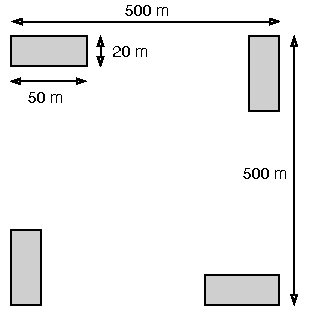
\includegraphics[width=0.5\textwidth]{schematic}
	\caption{Schematic diagram of plot layout within a site. Each 20x50 m (0.2 ha) plot is shaded grey. The site centre is denoted by a circle. Note that the plot dimensions are not to scale.}
	\label{schematic}
\end{figure}

Within each plot, the species of all trees with at least one stem $\geq$\stemSize{} cm DBH were recorded. Plot data was aggregated to the site level for analyses to avoid pseudo-replication caused by the more spatially coarse phenology data. Tree species composition varied little among the four plots within a site, and were treated as representative of the woodland in the local area. Using the Bray-Curtis dissimilarity index of species abundance data, we calculated that the mean pairwise compositional distance between plots within a site was lower than the mean compositional distance across all pairs of plots in \plotDistPer{}\% of cases.

To quantify phenology at each site, we used the MODIS MOD13Q1 satellite data product at 250 m resolution \citep{MOD13Q1}. The MOD13Q1 product provides an Enhanced Vegetation Index (EVI) time series at 16 day intervals. EVI is widely used as a measure of vegetation growth, as an improvement to NDVI (Normalised Differential Vegetation Index), which tends to saturate at higher values. Annual cumulative EVI is well-correlated with gross primary productivity and so can act as a suitable proxy \citep{}. We used all scenes from January 2015 to January 2021 with less than 20\% cloud cover covering the study area. All sites were determined to have a single annual growth season according to the MODIS VIPPHEN product \citep{}, which assigns pixels (0.05\textdegree, 5.55 km at equator) up to three growth seasons per year. We stacked yearly data between 2015 and 2020 and fit a General Additive Model (GAM) to produce an average EVI curve. We estimated the start and end of the growing season using first derivatives of the GAM. Start of the growing season was identified as the first day where the model slope exceeds half of the maximum positive model slope for a continuous period of \modisWin{} or more days, using only backwards looking data, following \citet{White2009}. Similarly, we defined the end of the growing season as the final day of the latest \trmmWin{} period where the GAM slope meets or exceeds half of the maximum negative slope. We estimated the length of the growing season as the number of days between the start and end of the growing season. We estimated the green-up rate as the slope of a linear model across EVI values between the start of the growing season and the point at which the slope of reduces below half of the maximum positive slope. Similarly the senescence rate was estimated as the slope of a linear model between the latest point where the slope of decrease fell below half of the maximum negative slope and the end of the growing season \autoref{ts_example}. We validated our calculations of cumulative EVI, mean annual EVI, growing season length, season start date, season end date, green-up rate and senescence rate with calculations made by the MODIS VIPPHEN product with linear models comparing the two datasets across our study sites (\autoref{vipphen_compare}, \autoref{annot_df}). We chose not to use the MODIS VIPPHEN product directly due to its more coarse spatial resolution (0.05\textdegree, 5.55 km at equator). Sites where our calculation of a phenological metric was drastically different to the MODIS VIPPHEN estimate were excluded, under the assumption that our algorithm had failed to capture the true value or some site specific factor precluded precise estimation. This removed \vipphenOutlier{} sites. 

Precipitation data was gathered using the ``GPM IMERG Final Precipitation L3 1 day V06'' dataset, which has a pixel size of 0.1\textdegree (11.1 km at the equator) \citep{GPM}, between 2015 and 2020. Daily total precipitation was separated into two periods: precipitation during the growing season (growing season precipitation), and precipitation in the 90 day period before the onset of the growing season (dry season precipitation). Rainy season limits were defined as for the EVI data, using the first derivative of a GAM to create a curve for each site using stacked yearly precipitation data, from which we estimated the half-max positive and negative slope to identify where the GAM model exceeded these slope thresholds for a consistent period of 20 days or more. Mean diurnal temperature range (Diurnal $\delta$T) was calculated as the mean of monthly temperature range from the WorldClim database, using the BioClim variables, with a pixel size of 30 arc seconds (926 m at the equator) \citep{Fick2017}. averaged across all years of available data (1970-2000). We calculated the lag between the onset of the growing season and the onset of the rainy season as the difference between these two dates as calculated above. We performed a similar calculation to estimate the lag between the end of the growing season and the end of the rainy season. 


\begin{figure}[H]
\centering
	\includegraphics[width=0.8\textwidth]{ts_example}
	\caption{Example EVI time series, demonstrating the metrics derived from it. Thin black lines show the raw EVI time series, with one line for each annual growth season. The thick black line shows the GAM fit. The thin blue lines show the minima which bound the growing season. The red line shows the maximum EVI value reached within the growing season. The shaded cyan area of the GAM fit shows the growing season, as defined by the first derivative of the GAM curve. The two orange dashed lines are linear regressions predicting the green-up rate and senescence rate at the start and end of the growing season, respectively. Note that while the raw EVI time series fluctuate greatly around the middle of the growing season, mostly due to cloud cover, the GAM fit effectively smooths this variation to estimate the average EVI during the mid-season period.}
	\label{ts_example}
\end{figure}

\subsection{Data analysis}

To measure variation in tree species composition we a used combination of Non-symmetric Correspondence Analysis (NSCA) and agglomerative hirerarchical clustering on species basal area weighted data \citep{Kreft2010, Fayolle2014}. NSCA was performed using the \texttt{ade4} R package \citep{ade4}. Scree plot analysis demonstrated that \nscaAxes{} axes was optimal to describe our data. These axes accounted for \nscaInertia{}\% of the variance in species composition according to eigenvalue decay. To guard against sensitivity to rare individuals, which can preclude meaningful cluster delineation across such a large species compositional range, we restricted the NSCA to species with five or more records, and to sites with more than five species \citep{}. We used Ward's algorithm to define clusters \citep{Murtagh2014}, based on the euclidean distance of sites in NSCA ordination space. We determined the optimal number of clusters by maximising the mean silhouette width among clusters \citep{Rousseeuw1987} \autoref{clust_sil}. Vegetation type clusters were used later as interaction terms in linear models. We described the vegetation types represented by each of the clusters using a Dufrene-Legendre indicator species analysis \citep{Dufrene1997}.

To describe the species diversity of each site, we calculated the Shannon-Wiener index ($H'$) from species basal area rather than individual abundance, as a measure of species richness effectively weighted by a species' contribution to canopy occupancy \citep{}. $H'$ was then transformed to the first order numbers-equivalent ($^1\!D$) of $H'$, calculated as $e^{H'}$ \citep{}. We use $^1\!D$ as the primary measure of species richness in our statistical models and is subsequently referred to as such. Additionally, we calculated a separate measure of abundance evenness, using the Shannon Equitability index ($E_{H'}$) \citep{Smith1996}. $E_{H'}$ was calculated as the ratio of basal area Shannon-Wiener diversity index to the natural log of total basal area per site.

We specified multivariate linear models to assess the role of tree species diversity on each of the chosen phenological metrics. We defined a maximal model structure including richness, abundance evenness, the interaction of richness and vegetation type, and climatic variables shown by previous studies to strongly influence phenology. The quality of the maximal model was compared to models with different subsets of independent variables using the model log likelihood, AIC (Akaike Information Criteria), BIC (Bayesian Information Criteria), and adjusted R\textsuperscript{2} values for each model. For each phenological metric, the best model according to the model quality statistics is reported in the results. Where two similar models were within 2 AIC points of each other, the model with fewer terms was chosen as the best model, to maximise model parsimony. All models were fitted using Maximum Likelihood (ML) to allow comparison of models \citep{}. The best model was subsequently re-fitted using Restricted Maximum Likelihood for model effect estimation (REML). Independent variables in each model were transformed to achieve normality where necessary and standardised to Z-scores prior to modelling to allow comparison of slope coefficients within a given model.

We used the \texttt{ggeffects} package to estimate the marginal means of the interaction effect of species diversity and vegetation type, to investigate vegetation type specific effects on each phenological metric \citep{ggeffects}. Estimated marginal means entails generating model predictions across values of a focal variable, in this case species diversity, while holding non-focal variables constant. All statistical analyses were conducted in R version 4.0.2 \citep{R2020}.

\section{Results}

Model selection showed that richness and evenness are important determinants of each of the chosen phenological metrics, across vegetation types. The effect of richness featured and was significant in all best models except for senescence laf and senescence rate. Evenness was a significant effect in models for cumulative EVI, season length and senescence lag only \autoref{mod_slopes}.

\nCluster{} vegetation type clusters were identified during hierarchical clustering. Cluster 3, which contains the most sites (\nClusterC{}), consists of small stature Zambesian woodlands, as referenced by \citet{Dinerstein2017} and \citet{Chidumayo2001}, and is not dominated by a particular large canopy tree species. It is possible that these woodlands represent highly disturbed woodlands where large trees may have been removed by humans. Abundance evenness is high across sites in Cluster 3. Cluster 2 is dominated heavily by \textit{Brachystegia boehmii}, while Cluster 1 is dominated by \textit{Julbernardia paniculata}, both large canopy-forming trees. These two clusters likely represent variation among miombo woodland types in dominant canopy tree species. Both Clusters 1 and 2 have a similar composition of non-dominant smaller shrubby species, such as \textit{Pseudolachnostylis maprouneifolia} (\autoref{clust_summ}).

As expected (H\textsubscript{3}), richness and wet season precipitation both had positive significant effects on cumulative EVI and season length. In contrast, abundance evenness, the other aspect of tree species diversity in our models, had a significant negative effect on both cumulative EVI and season length (\autoref{mod_slopes}).

Species richness caused a significant increase in the lag time between date of green-up and date of rainy season onset (H\textsubscript{2}). This effect was comparable to the effects of pre-season precipitation and diurnal temperature range, which also caused an increase in green-up lag. In contrast, senescence lag was poorly defined by our models, suggesting that some unmeasured factor remains the key driver of this phenological metric. The effects of diurnal $\delta$T and abundance evenness had wide confidence interval. The best model explained only 1\% of the variance in senescence lag, though was still better quality than a climate-only model.

All best models including tree species diversity variables were of better quality than models which included only climatic variables \autoref{mod_stat}. The phenological metrics best predicted were green-up lag and cumulative EVI, where models explained 26\% and 34\% of the variance in these variables, respectively. Senescence rate and senescence lag were the least well predicted phenological metrics, with the best model explaining 3\% and 2\% of their variance, respectively.

While species richness had a significant negative effect on green-up rate, as predicted by H\textsubscript{1}, the best model, which also included pre green-up precipitation and diurnal temperature range, only explained 10\% of the variance in this metric. 

The slope of the relationship between species richness and phenological metrics varied among vegetation types, but maintained the same direction in all cases except rates of green-up and senescence \autoref{mod_marg}. Across all models however, none of the vegetation types were significantly different, according to post-hoc Tukeys's tests on marginal effects (\autoref{lsq_terms}). Clusters were largely similar in their density distribution of the six phenological metrics \autoref{phen_dens_clust}. The most striking differences are the presence of some sites in Cluster 3 with particularly high green-up rates. The hierarchical clustering analysis demonstrated that there was little spatial structure to the vegetation clusters identified. The key emergent trend was that Cluster 2 was absent from the southwest of the country (\autoref{plot_loc}) possibly due to the low levels of precipitation in this region, which could preclude many miombo tree species.

\input{out/clust_summ.tex}

\input{out/mod_stat.tex} 

\begin{figure}[H]
\centering
	\includegraphics[width=\textwidth]{mod_slopes.pdf}
	\caption{Standardized slope coefficients for each best model of a phenological metric. Slope estimates are $\pm$1 standard error. Slope estimates where the interval (standard error) does not overlap zero are considered to be significant effects.}
	\label{mod_slopes}
\end{figure}

\begin{figure}[H]
\centering
	\includegraphics[width=\textwidth]{mod_marg.pdf}
	\caption{Marginal effects of tree species richness on each of the phenological metrics, for each vegetation type, using the best model including the interaction of species richness and vegetation cluster, for each phenological metric.}
	\label{mod_marg}
\end{figure}

\begin{figure}[H]
\centering
	\includegraphics[width=\textwidth]{nsca.pdf}
	\caption{Plot scores of the (A) first and second, and (B) third and fourth axes of the Non-Symmetric Correspondence Analysis of tree species composition. Points are coloured according to clusters defined by Ward's algorithm on euclidean distances of the NSCA ordination axes, along with a convex hull encompassing 95\% of the points in each cluster.}
	\label{nsca}
\end{figure}

\begin{figure}[H]
\centering
	\includegraphics[width=\textwidth]{phen_dens_clust}
	\caption{Density distribution of the six phenological metrics used in the study, grouped by vegetation type cluster. For a pairwise comparison of phenological metrics and their correlations, see \autoref{phen_bivar} and \autoref{phen_bivar_corr}.}
	\label{phen_dens_clust}
\end{figure}

\section{Discussion}

In this study we have demonstrated a clear and measurable effect of tree species richness across various aspects of land-surface phenology in Zambian deciduous savannas. We showed that tree species richness led to an increase in cumulative EVI and season length. Additionally, species richness led to a slower rate of greening and caused the onset of greening to occur earlier with respect to the start of the rainy season. Our study lends support for a positive biodiversity - ecosystem function relationship in our chosen study area, operating through its influence on phenology. Our results exemplify the key role of tree species biodiversity in driving key ecosystem processes, which affect ecosystem structure, the wildlife provisioning role, and the gross primary productivity of ecosystems.

Our finding that species richness strongly affects patterns of land-surface phenology in deciduous savannas has important consequences for two pertinent fields of ecological research. Firstly, it should prompt conservation scientists to take advantage of remotely sensed land-surface phenology data to improve estimates of tree species diversity. The technology behind remote-sensing of tree species diversity is maturing fast, providing a means to rapidly and accurately assess the conservation priority of biodiversity hotspots, and to identify regions suffering biodiversity loss. Secondly, it can provide earth surface system modellers with a means to better understand how future changes in species diversity and composition will affect land-surface phenology and therefore the carbon cycle. Incorporating predictions of biotic change into carbon models has been slow, owing to large uncertainties in the effects of diversity on Gross Primary Productivity (GPP). Our study provides a link by demonstrating a strong positive relationship between species richness and EVI, which itself drives GPP.

Patterns of senescence were poorly predicted by species richenss and evenness in our models. \citet{Cho2017} found that tree cover, measured by MODIS LAI data, had a significant effect on senescence rates in savannas in South Africa, which have similar climatic conditions to the sites in our study. In sparse savannas, while the onset of the growing season is often driven by tree photosynthetic activity, which may precede the onset of precipitation, the end of the growing season is conversely driven by grasses \citep{}. Grass activity is much more reactive to short-term changes in soil moisture than tree activity, and may oscillate within the senescence period. This may explain the lack of a strong precipitation signal for senescence lag and senescence rate. Other studies both global and within southern African savannas have largely ignored patterns of senescence, instead focussing patterns of green-up \citep{Gallinat2015}. Most commonly, these studies simply correlate the decline of rainfall with senescence, but the lack of precipitation as a term in our best model suggests that other unmeasured factors are at play. Alternatively, \citet{Zani2020} suggests that in resource limited environments, senescence times may largely be set by the preceding photosynthetic activity and sink-limitations on growth. For example, limited nutrient supply may prohibit photosynthesis late in the season if the preceding photosynthetic activity has depleted that supply. \citet{Reich1992} suggested that there may be direct constraints on leaf life-span, especially in disturbance and drought-prone environments such as those studied here, which would lead to senescence rate being set largely by the time since bud-burst. In our study however, we found that there was variation in season length between plots, indicating that there are additional factors at play. 

While leaf senescence is not as important for the survival of browsing herbivores as green-up, the timing of senescence with respect to temperature and precipitation has important consequences for the savanna understorey microclimate. The longer leaf material remains in the canopy after the end of the rainy season, the greater the microclimatic buffer for herbaceous understorey plants and animals, which require water and protection from high levels of insolation and dry air which can prevail rapidly after the end of the rainy season \citep{}. Our study merely exemplifies that more work needs to be done to properly characterise the drivers of senescence in this biome.

While species richness is a common measure of biodiversity, abundance evenness constitutes a second key axis \citep{Wilsey2005, Hillebrand2008}. While traditionally species richness and evenness were assumed to be highly positively correlated, recent work has demonstrated that in many systems, richness and evenness may be nearly orthogonal \citep{}. In this study, we found contrasting effects of richness and evenness on both cumulative EVI and season length. Evenness caused a decrease in these phenological metrics, which we did not expect. It is possible that the negative effect of abundance evenness occurred because an increase in evenness is associated with a reduction in the canopy cover of a few highly dominant large canopy tree species (e.g. \textit{Brachystegia boehmii} and \textit{Julbernardia paniculata}), as part of the transition from woody savanna to thicket vegetation, or following a major disturbance event. Large canopy tree species have access to ground water for a longer part of the year, due to their deep root systems and conservative growth patterns. A future study may choose to explore the differential effects of species diversity in different size classes and in different physiognomic groups defined by functional form, e.g. shrub, canopy tree, coppicing tree.

Our coverage of very short season lengths in Zambia, as estimated by the VIPPHEN product, was restricted, with notable absences of plot data in the northeast of the country around 30.5\textdegree{}E, 11.5\textdegree{}S, and 23.0\textdegree{}E, 15.0\textdegree{}S. Upon further inspection of true colour satellite imagery, these regions are largely seasonally water-logged floodplain and swampland, and were likely ignored by the ILUA-II assessment for this reason. This also explains their divergent phenological patterns as observed in the MODIS EVI data. 

It is important to note that the remotely sensed EVI measurements used here aren't specific only to trees, they represent the landscape as a singe unit. Nevertheless, seasonal patterns of tree leaf phenology in southern African deciduous woodlands, particularly the pre-rainy season green-up phenomenon, is driven almost exclusively by trees, while grasses tend to follow patterns of precipitation more closely \citep{}. Grasses contribute to gross primary productivity, and it was therefore in our interests to include their response in our analysis as we seek to demonstrate how tree species richness can affect cycles of carbon exchange. Additionally, the micro-climatic effects of tree leaf canopy coverage and hydraulic lift through tree deep root systems will benefit the productivity of grasses as well as understorey tree individuals.

It is possible that not all tree individuals in our dataset exhibited a completely deciduous growth pattern. Some highly conservative species in this region remain evergreen throughout the dry season. \todo{MORE}.

\section{Conclusion}

Here we explored the role of tree species diversity on land surface phenology across Zambia. We showed that species richness clearly affects rate of green-up, the lag time between rainy season onset and growth, and the length of the growing season. Our results have a range of consequences for earth system mdoellers and conservation managers, and lend further support to an already well established corpus of the positive effect of species diversity on ecosystem function.

\printbibliography

\section{Supplementary Material}
\beginsupplement

\begin{figure}[H]
\centering
	\includegraphics[width=\textwidth]{vipphen_compare}
	\caption{Scatter plots showing a comparison of phenological metrics from the MODIS VIPPHEN product \citep{VIPPHEN} and those extracted from the MOD13Q1 data \citep{MOD13Q1}, for each of the sites in our study. The cyan line shows a linear model of the data, with a 95\% confidence interval.}
	\label{vipphen_compare}
\end{figure}

\input{out/vipphen_compare.tex}

\begin{figure}[H]
\centering
	\includegraphics[width=\textwidth]{phen_bivar}
	\caption{Scatter plots showing pairwise comparisons of the six phenological metrics used in this study, extracted from the MODIS MOD13Q1 product \citep{MOD13Q1}. Points represent study sites and are coloured by vegetation type. Linear regression line of best fit for all sites is shown as a black line, while linear regressions are shown for each vegetation type cluster as coloured lines.}
	\label{phen_bivar}
\end{figure}

\input{out/all_mod_sel.tex}

\begin{figure}[H]
\centering
	\includegraphics[width=\textwidth]{img/clust_sil.pdf}
	\caption{Mean silhouette width for agglomerative hierarchical clustering, specifying a varying number of clusters. The highest silhouette width, and therefore the number of clusters chosen in our analysis, is denoted by a dashed line.}
	\label{clust_sil}
\end{figure}

\begin{figure}[H]
\centering
	\includegraphics[width=\textwidth]{img/clust_dendro.pdf}
	\caption{Dendrogram of hierarchical clustering of euclidean distances of NSCA (Non-Symmetric Correspondence Analysis) ordination axes, clustered using the Ward algorithm. Clusters are denoted by coloured boxes.}
	\label{clust_dendro}
\end{figure}

\input{out/lsq_terms_fmt.tex}

\end{document}

